\section{Introduction}

%\subsection{White Rabbit}

White Rabbit (WR)~\cite{biblio:whiteRabbit} is a technology based on existing standards, namely
Ethernet (IEEE~802.3) \cite{biblio:IEEE8023}, Synchronous Ethernet (SyncE) \cite{biblio:SynchE}
and IEEE~1588 (PTP)~\cite{biblio:IEEE1588}, which enables sub-nanosecond synchronization of 
thousands of devices connected in a network spanning several kilometers. In addition to high-accuracy 
timing capabilities, a WR network features low-latency, reliable and deterministic data delivery 
\cite{biblio:ICALEPCS2011}.

Sub-nanosecond accuracy and picosecond precision (jitter) of time distribution in a WR network is 
achieved by both extending and hardware-supporting PTP to address its limitations. The WR extension to PTP
is called WRPTP. It is defined in the form of a PTP Profile \cite{biblio:ISPCS2011} and described in the 
WR Specification~\cite{biblio:WRPTP}. WRPTP uses SyncE to distribute the common notion of 
frequency in the entire network over the physical medium. \modified{By having hardware syntonization}
it casts the problem of timestamping 
into a phase detection measurement using Digital Dual Mixer Time Difference (DDMTD) 
\cite{biblio:DDMTD}\cite{biblio:WRproject}. The results of these precise measurements are used both during 
normal PTP operation and for quantifying physical medium asymmetry during the calibration phase 
\cite{biblio:TomekMSc}.

WR, originally started as a successor of the current control and timing network at 
CERN (General Machine Timing)~\cite{biblio:GMT}, is now a multi-laboratory and multi-company 
effort with many potential scientific and commercial applications. Apart from the application
for accelerators (i.e.: CERN~\cite{biblio:WRproject}, GSI~\cite{biblio:FAIRtimingSystem}),
WR is also considered a good candidate as a synchronization and acquisition system for 
cosmic particle detectors (e.g.:~LHAASO~\cite{biblio:LHAASO}, KM3NeT~\cite{biblio:KM3NeT}) or long distance 
time transfer systems \cite{biblio:TWTFT}. Time transfer in the CERN Neutrinos to Gran Sasso (CNGS) 
project is the first application for which WR is deployed. 

In this paper we describe the CNGS project (Section~\ref{sec:CNGS}) focusing on the 
WR installation, monitoring and test setups (Section~\ref{sec:deplAndMeas}). 
Then we analyze the collected data in Section~\ref{sec:dataAnalysis} and finish with conclusions
in Section~\ref{sec:conclusions}.

% The CNGS Project is introduced shortly below (Section~\ref{sec:CNGS}). The WR installation in 
% CERN and Gran Sasso National Laboratory (LNGS) along with the measurement setup are described in 
% Section~\ref{sec:deplAndMeas}. Next section analyzes the collected long-term measurement data 
% of WR performance. Finally, conclusions are presented in the last section.


\section{CERN Neutrinos to Gran Sasso (CNGS)}
\label{sec:CNGS}

\begin{figure}[!t]
\centering
%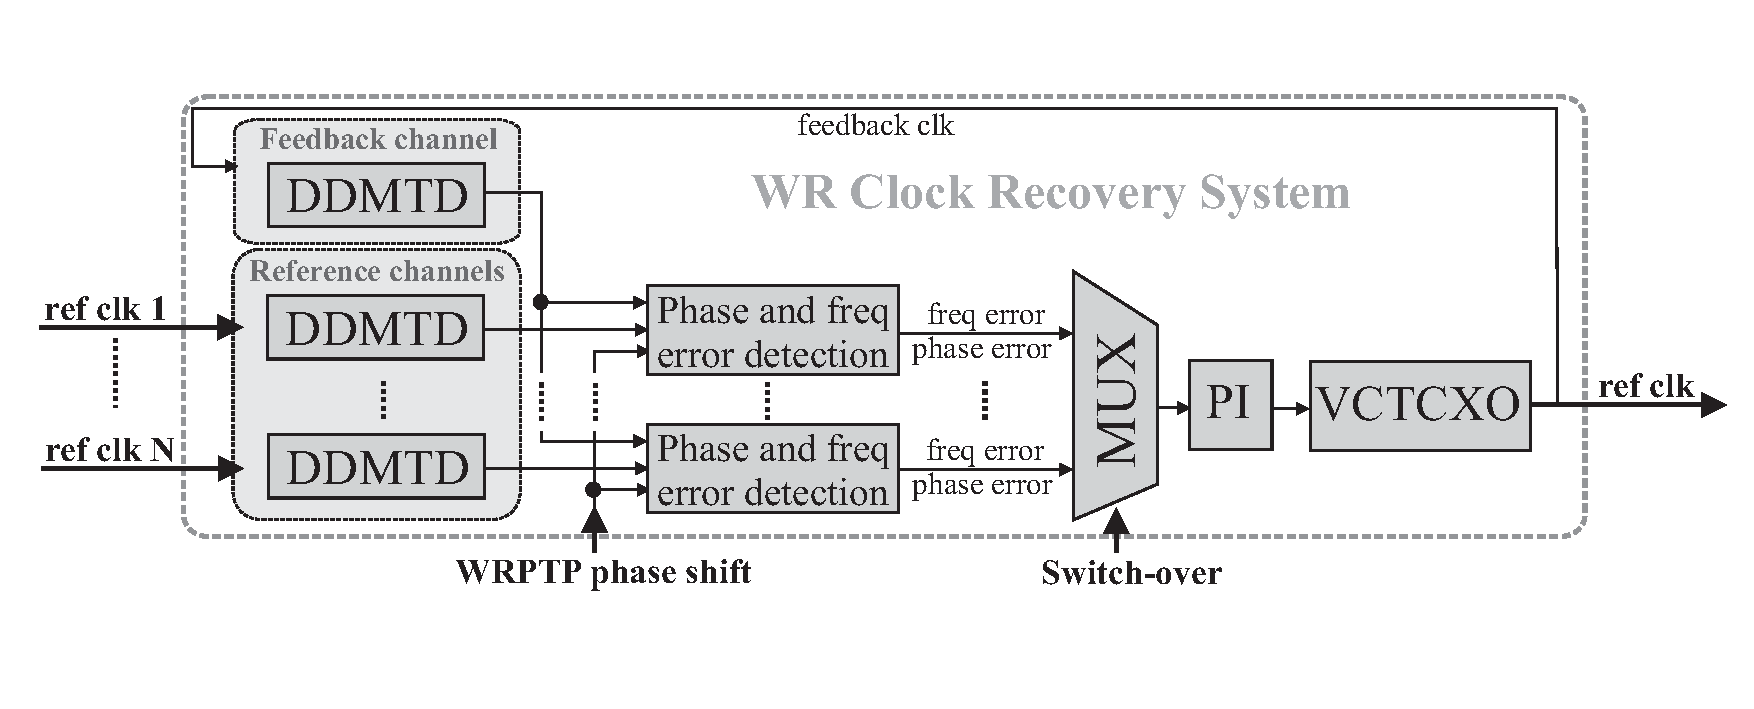
\includegraphics[width=2.95in]{fig/wrCRS.eps}
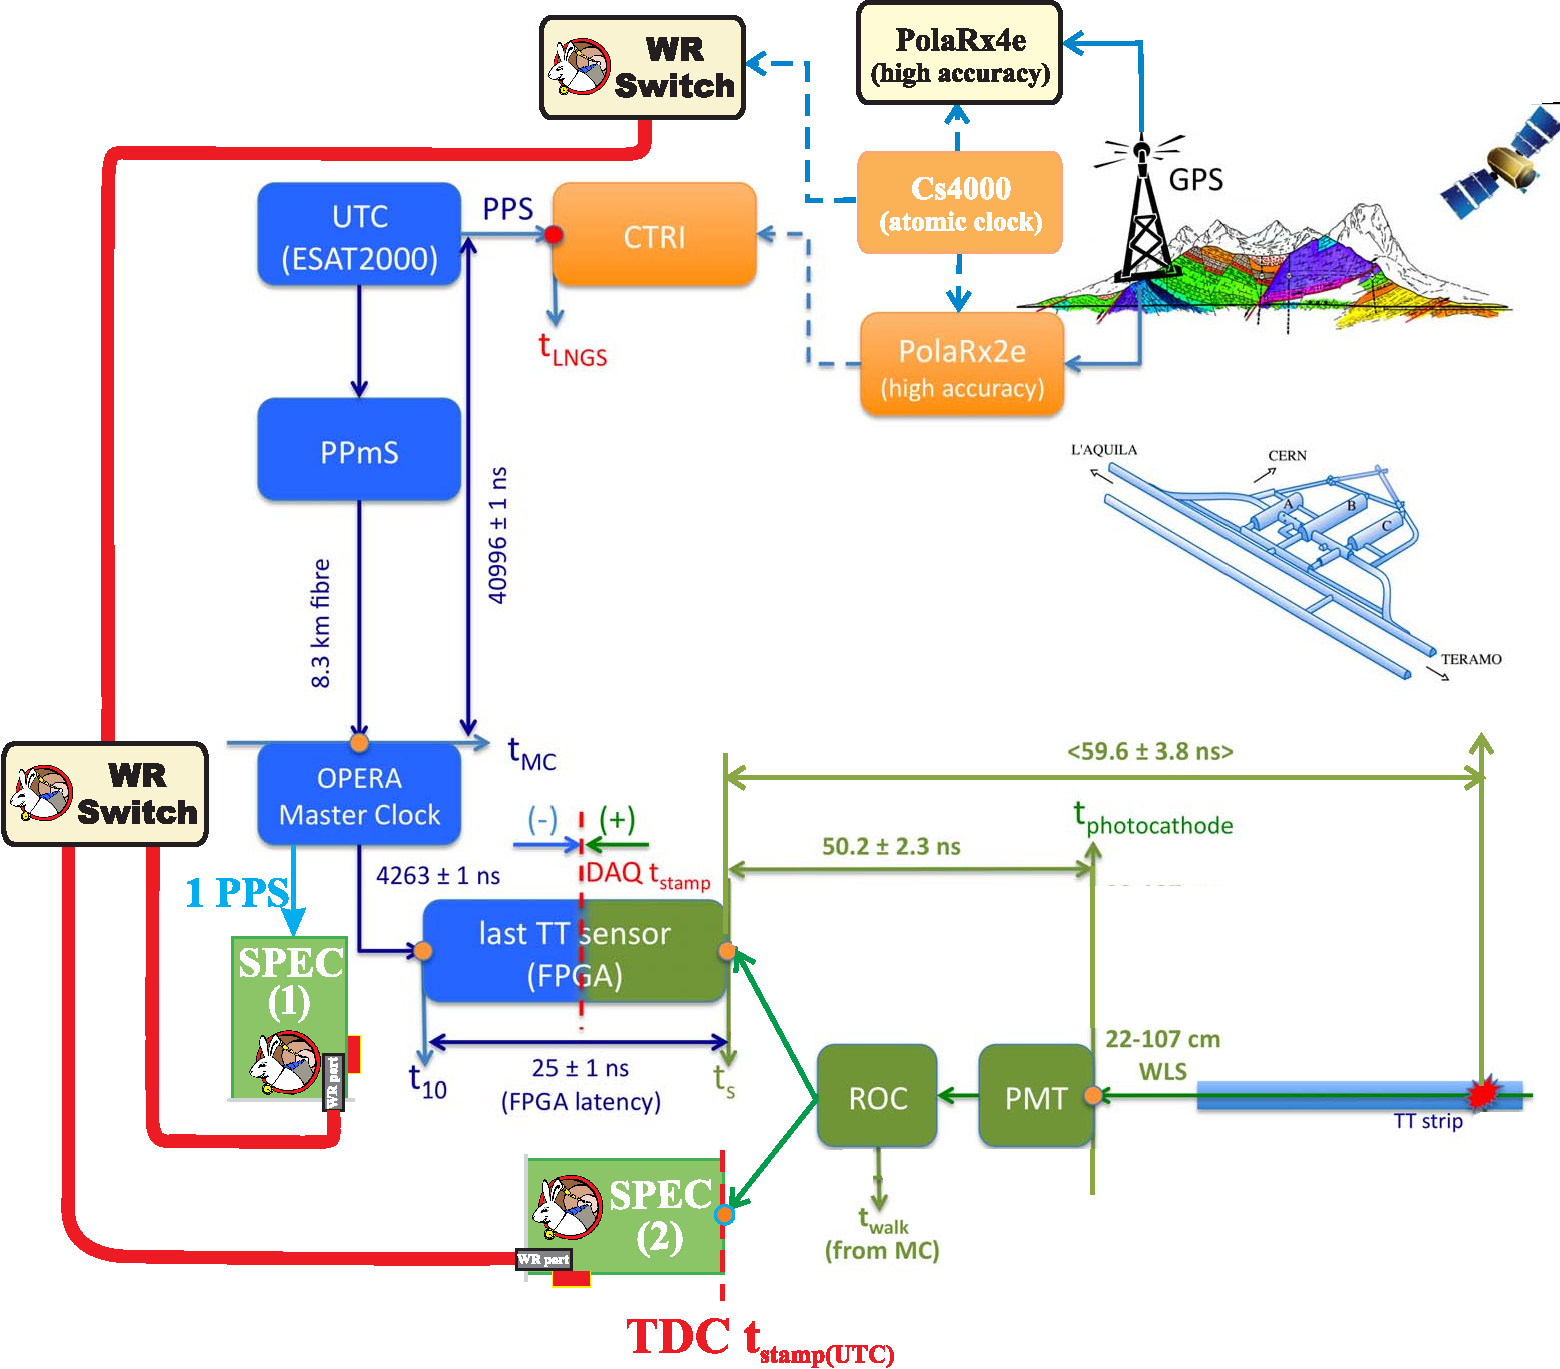
\includegraphics[height=2.9in]{../../figures/applications/OperaTiming2.eps}
\caption{Schematic of the OPERA timing system at LNGS. Blue delays include elements of the 
timestamp distribution. Green delays indicate detector time-response. 
Orange boxes refer to elements of the old CNGS-OPERA synchronization system (\cite{biblio:TOF}). 
WR Switches, SPECs and PolaRx4e are the elements of the new installation.}
\label{fig:operaTiming}
\end{figure}


The CNGS project \cite{biblio:CNGS2000} consists of the production of a neutrino beam at CERN and sending
it towards the Gran Sasso National Laboratory (LNGS). The project employs a GPS-based CERN-LNGS 
synchronization \cite{biblio:BECOHT_CNGS} to enable discrimination in LNGS detectors between 
neutrinos coming from the Sun (or other sources) and those coming from the CNGS beam. 
% The very high 
% precision (a few nanoseconds) of such synchronization opened the way to meaningful neutrino 
% Time Of Flight (TOF) measurements \cite{biblio:TOF} in years 2009, 2010 and 2011.
%Needing 
\modified{The need for} nanosecond accuracy between the GPS receivers located at CERN and LNGS is only a part of the 
CERN-LNGS time transfer \modified{challenge. Moreover}, a similar degree of accuracy needs to be 
%achieved
\modified{established} in 
calibrating cabling lengths and device delays between the GPS receivers and the points where
the measurements are actually taken. 

A common UTC timebase for both remote sites \attention{has} been achieved so far using two identical 
systems, composed of a Septentrio PolaRx2e \cite{biblio:PolaRx2e} GPS receiver operating in 
``common-view" mode and a Symmetricom Cs4000 \cite{biblio:CS4000} \modified{Cesium (Cs)} atomic clock, installed at 
CERN and LNGS. The nanosecond level of accuracy of this setup has been successfully verified by 
independent measurements \cite{biblio:TOF}. 

The synchronization between the UTC timebase at the GPS receiver and the measurement point \attention{has}
been performed so far using the General Machine Timing at CERN and the detector timing system 
(e.g~OPERA's) at LNGS. High accuracy in these systems \attention{is} achieved by hand-evaluating delays introduced 
by each element of the timing systems at CERN and LNGS using the methods described in 
\cite{biblio:TOF} and \cite{biblio:BECOHT_CNGS}. 
\figurename~\ref{fig:operaTiming} depicts the synchronization of the OPERA \cite{biblio:TOF} 
detector (orange and blue boxes) and the delays introduced by each of its elements. 

Additionally to the system described above and used since 2009, a new WR-based system 
(\figurename~\ref{fig:wrLNGStiming}) was installed at CERN and LNGS in May 2012. This new 
installation
% enables to unify 
\modified{unified} the entire CERN-LNGS time transfer chain
(so far it \modified{had been} identical only from GPS to GPS). 
%It is meant to 
\modified{Its purpose is to} verify 
the performance of the old installation and further enhance the accuracy of the CERN-LNGS 
time transfer. 
%This WR installation is described in the next section. 



% Before White Rabbit installation, the synchronization between UTC time base at GPS receivers and 
% measurement points was achieved by hand-evaluating delays introduced by each element of the timing 
% systems at CERN and LNGS using methods described in \cite{biblio:TOF} and \cite{biblio:BECOHT_CNGS}. 
% \figurename~\ref{fig:operaTiming} depicts synchronization of the OPERA \cite{biblio:TOF} detector 
% and delays introduced by each of its elements. Additionally, the new White Rabbit installation 
% is presented in the figure to indicate its role in the synchronization. Both systems are running
% in parallel. 








% which require high accuracy of the relative time tagging at CERN and 
% detectors located at LNGS. 

% The achieved high precision of synchronization (systematic uncertainty at the leve of several 
% nanoseconds) between the extraction line at CERN and detector at LNG opened the way to meaningful 
% ne

